\begin{comment}
    

%\addtocounter{chapter}{-1}
\chapter[\textit{Resultados teóricos y experimentales}]{Resultados teóricos y experimentales}
\begin{flushright}
\textsc{Presenta un análisis teórico del comportamiento del torque y las pérdidas de la máquina junto con los resultados de las pruebas en entorno controlado y de rodamiento en un trayecto predefinido.}
\end{flushright}
\label{chap:capitulo4}


\vfill
\renewcommand{\mtctitle}{Contenido}
\minitoc
\newpage
\end{comment}


\section{Capitulo 5: Análisis Comparativo de las Técnicas Implementadas}


En esta sección se presenta un análisis comparativo de las técnicas de diseño de UNS implementadas en la plataforma de entrenamiento IIoT con los métodos propuestos por Schultz y Parris. Ambos enfoques han sido desarrollados bajo la misma plataforma IIoT, utilizando el protocolo MQTT Sparkplug B, lo que permite evaluar de manera objetiva las diferencias y ventajas que ofrece cada uno en términos de métricas de rendimiento dentro de un entorno industrial y académico que se definirán durante el desarrollo de esta sección. 

El objetivo principal de este análisis es identificar las fortalezas y limitaciones de cada técnica en la representación de la arquitectura UNS, considerando métricas de desempeño cuantitativos y cualitativos como se muestra en la tabla \ref{clas_metricas}. Allí se detallan métricas como cantidad de mensajes, autenticaciones, clientes, tópicos, además de características como la resiliencia de la arquitectura, la facilidad de integración de nuevos dispositivos y la flexibilidad para adaptarse a distintos sistemas y plataformas IIoT.


\begin{table}[H]
\centering
\begin{tabular}{|c|c|c|c|}
\hline
\textbf{Tipo} & \textbf{Métrica} & \textbf{Tipo} & \textbf{Métrica} \\
\hline
\multirow{Cuantitativas} & Gestión de Tópicos y Sesiones MQTT & \multirow{Cualitativas} & Integración \\
\cline{2-2} \cline{4-4}
 & Gestión de Autenticaciones y Autorizaciones &  & Resiliencia \\
\cline{2-2} \cline{4-4}
 & Flujo de Datos &  & Flexibilidad \\
\cline{2-2} \cline{4-4}
 & Gestión de Clientes &  & Seguridad \\
\cline{2-2} \cline{4-4}
 & Gestión de Mensajes &  & Implementación \\
\cline{2-2} \cline{4-4}
 & Actividad de Paquetes &  & Escalabilidad\\
\hline
\end{tabular}
\caption{Clasificación de Métricas de Desempeño}
\label{clas_metricas}
\end{table}


Las métricas de evaluación fueron seleccionadas con base en su capacidad de medición, su aplicabilidad dentro de la plataforma y el impacto que generan en ella. Además, se consideró la experiencia previa en su uso y el contexto en el que se implementan, lo que permitió identificar el enfoque más adecuado según los requerimientos específicos.



\subsection{Métricas Cualitativas de Desempeño}

Las métricas cualitativas seleccionadas para el análisis comparativo responden a criterios fundamentales que determinan la viabilidad, robustez y sostenibilidad de una arquitectura IIoT en entornos industriales complejos. Estas métricas permiten evaluar el esfuerzo requerido en el proceso de desarrollo e integración, además de la adaptabilidad del sistema ante fallos, la facilidad para incorporar nuevos componentes, la compatibilidad con tecnologías existentes, el cumplimiento de requisitos de seguridad y la capacidad de crecimiento estructurado del sistema. En este sentido, estas dimensiones representan aspectos críticos que influyen directamente en la eficiencia operativa y en la toma de decisiones al momento de seleccionar una arquitectura IIoT adecuada para entornos reales de despliegue.

La elección de las métricas de capacidad de implementación, resiliencia de la arquitectura, flexibilidad, seguridad, facilidad de integración y escalabilidad obedece a su capacidad de capturar de manera integral las fortalezas y limitaciones de cada técnica desde una perspectiva técnica, operativa y estratégica. Cada una de estas dimensiones ofrece una visión complementaria sobre el comportamiento del sistema bajo distintas condiciones de operación, lo que permite establecer una comparación estructurada entre ambas técnicas. A continuación, se detalla el análisis individual de cada métrica, indicando para cada caso cuál de las dos técnicas presenta mayores ventajas.

\subsubsection{Integración}
La técnica de Parris se distingue por su enfoque directo en la construcción del UNS, donde cada uno de los Path correspondientes a la jerarquía definida se configura individualmente en los dispositivos de cada Plataforma IIoT. Todos los Path son publicados hacia un único broker MQTT centralizado, lo que permite que cualquier aplicación conectada al broker (sistemas SCADA, dashboards o bases de datos) pueda consumir los datos sin necesidad de procesos intermedios. Esta simplicidad en la arquitectura y la menor cantidad de capas intermedias facilitan la integración, reduciendo el esfuerzo en la configuración inicial y permitiendo una rápida puesta en marcha con conocimientos técnicos moderados.

En contraste, la técnica de Schultz exige una integración jerárquica estructurada que incluye la configuración de nodos UNS a nivel de \textit{Area}, \textit{Site} y \textit{Enterprise}. Cada uno de estos niveles requiere instancias separadas que actúan como agregadores y modeladores de datos, lo que demanda una infraestructura de TI más robusta y mayor coordinación entre equipos de trabajo. Además, esta técnica implica un conocimiento avanzado sobre comunicación entre brokers, estructuras de tópicos intermedios y manejo de conexiones distribuidas, lo que eleva la complejidad general del despliegue. En consecuencia, la técnica de Parris se posiciona como la opción más sencilla y eficiente en términos de integración, especialmente en entornos donde se busca una solución rápida, flexible y de bajo costo de entrada.

\subsubsection{Resiliencia}
En el contexto de arquitecturas IIoT, la resiliencia se refiere a la capacidad del sistema para mantener la operatividad y disponibilidad de los servicios ante fallos, interrupciones o desconexiones parciales o totales. Esta métrica es crucial cuando se diseñan sistemas distribuidos para entornos industriales, donde la continuidad operativa es esencial y cualquier caída puede tener consecuencias significativas a nivel de producción o monitoreo.

La técnica de Schultz presenta una ventaja clara en este aspecto, ya que su diseño se basa en una arquitectura distribuida con múltiples niveles de brokers MQTT independientes, organizados por \textit{Area}, \textit{Site} y \textit{Enterprise}. Esto permite que, en caso de una falla localizada en un broker de \textit{Site} o broker de \textit{Area}, el resto del sistema continúe funcionando sin afectación. Cada nivel actúa como una unidad autónoma de comunicación, lo que otorga tolerancia a fallos y segmentación natural del riesgo.

Por el contrario, la técnica de Parris depende de una estructura centralizada donde todos los dispositivos publican directamente hacia un único broker MQTT en la nube. Esta centralización implica que cualquier interrupción del broker o de la conectividad hacia la nube impacta inmediatamente a toda la infraestructura, afectando a todos los \textit{Sites}, \textit{Areas} y \textit{Lines} conectadas. No existen mecanismos nativos de aislamiento ante fallos, lo que limita su resiliencia en escenarios de redes inestables o entornos críticos. En consecuencia, la técnica de Schultz es claramente superior en términos de resiliencia, ya que ofrece una arquitectura distribuida y segmentada que proporciona mayor robustez operativa ante fallos de red o caídas puntuales en la infraestructura.

\subsubsection{Flexibilidad}
Esta métrica se conoce como la capacidad del sistema para adaptarse fácilmente a distintos entornos tecnológicos, aplicaciones externas y cambios en la infraestructura, permitiendo la interoperabilidad con diversas plataformas y facilitando el acceso a la información desde diferentes puntos del ecosistema industrial.

En este sentido, la técnica de Parris demuestra una mayor flexibilidad operativa. Su arquitectura centralizada permite que cualquier aplicación o sistema que soporte el protocolo MQTT, ya sea una plataforma IIoT, un sistema SCADA o un visualizador como Grafana, pueda conectarse directamente al broker para consumir la información, sin necesidad de intermediarios adicionales. Esta independencia amplía significativamente las posibilidades de integración con tecnologías de terceros en la nube y en entornos locales.

Por el contrario, la técnica de Schultz presenta limitaciones importantes en este aspecto. Su diseño jerárquico requiere la implementación de plataformas IIoT industriales como Ignition en cada uno de los niveles del UNS para consolidar y enviar los datos. Esto no solo implica una mayor inversión en infraestructura, sino que también restringe la compatibilidad con aplicaciones externas, ya que estas no pueden acceder directamente al flujo de datos sin pasar por las capas intermedias. Por lo tanto, en términos de interoperabilidad y adaptabilidad, la técnica de Parris resulta más flexible, al simplificar la conexión de nuevas aplicaciones y permitir un acceso más abierto y directo a la información industrial.

\subsubsection{Seguridad}
La capacidad para proteger la integridad, confidencialidad y disponibilidad de los datos a lo largo de toda la infraestructura define la seguridad del sistema. Esto incluye la gestión de accesos, la segmentación de redes, el control de usuarios y la protección contra amenazas tanto internas como externas. 

Desde este enfoque, la técnica de Schultz ofrece una arquitectura inherentemente más robusta en términos de seguridad. Al implementar una jerarquía distribuida de brokers MQTT en los distintos niveles del UNS, es posible definir políticas de autenticación y autorización específicas para cada nodo de la red. Esto permite aplicar controles de acceso diferenciados en función del rol del usuario o del sistema cliente, así como segmentar los datos según su criticidad. Además, la descentralización facilita la contención de incidentes, es decir, una brecha de seguridad en un área no compromete al resto de la infraestructura, ya que los brokers funcionan de forma independiente.

Por el contrario, la técnica de Parris se basa en un modelo centralizado en el que toda la información fluye hacia un único broker MQTT. Aunque este broker puede protegerse mediante autenticación con credenciales, certificados y cifrado TLS, el punto único de acceso concentra todo el tráfico y la información del sistema, lo que lo convierte en un objetivo más vulnerable ante posibles ataques o fallos de configuración. Una vez establecida la conexión, los clientes autenticados tienen acceso a la totalidad del flujo de datos. En consecuencia, la técnica de Schultz representa una solución más segura, al permitir una segmentación más fina de los permisos, una gestión descentralizada de los accesos y una mayor capacidad de aislamiento ante incidentes.

\subsubsection{Implementación}
El nivel de esfuerzo técnico y operativo necesario para conectar distintas aplicaciones, plataformas y servicios dentro de una arquitectura IIoT es otro criterio a tener en cuenta. Se requiere asegurar que los datos puedan ser consumidos y comprendidos de manera estructurada y eficiente por los diferentes componentes del sistema.

En este aspecto, la técnica de Schultz presenta una implementación más directa y estructurada, ya que la segmentación de los niveles del UNS es gestionada automáticamente por la propia plataforma IIoT (Ignition). Esta jerarquía se construye conforme se interconectan los distintos brokers MQTT en cada nivel, lo que permite a los usuarios trabajar con rutas de datos ya organizadas y comprensibles desde el punto de vista de la arquitectura definida. 

Por el contrario, en la técnica de Parris, a pesar de la centralización de la información en un único broker, la estructuración jerárquica del UNS debe realizarse de manera manual. Es necesario definir cada uno de los Path de publicación, estableciendo el uso de delimitadores (como el guion bajo \textbf{“\_”}) que posteriormente deberán ser interpretados por las aplicaciones consumidoras. Este enfoque implica un mayor conocimiento técnico en programación, manejo de estructuras de nodo y un entendimiento profundo de la lógica jerárquica del UNS, lo que puede dificultar la implementación en entornos con múltiples fuentes de datos y usuarios no especializados. Por estas razones, la técnica de Schultz ofrece una mayor facilidad de implementación, al delegar la segmentación jerárquica a la lógica propia de las plataformas IIoT utilizadas, reduciendo así la complejidad técnica para el usuario final.

\subsubsection{Escalabilidad}
La escalabilidad evalúa la facilidad con la que una arquitectura IIoT puede crecer incorporando nuevos dispositivos o casos de estudio sin re-configuraciones complejas. Esta métrica implica corporar nuevos dispositivos, sensores, plataformas o casos de estudio, manteniendo siempre una lógica coherente y eficiente de integración de datos. 

La técnica de Schultz se destaca al permitir que, al añadir nuevos elementos, estos se integren directamente al nivel jerárquico correspondiente del UNS, actualizando automáticamente toda la infraestructura sin necesidad de modificaciones manuales. Por el contrario, Parris requiere definir manualmente nuevos Path y adaptar la plataforma IIoT para nivel del UNS, lo que incrementa la complejidad y el riesgo de errores. En este sentido, Schultz ofrece una escalabilidad superior, siendo más eficiente y robusta frente al crecimiento del sistema.

    

\subsection{Métricas Cuantitativas de Desempeño}

Para complementar el análisis comparativo entre las técnicas de diseño de UNS, se definieron un conjunto de métricas cuantitativas de desempeño orientadas a evaluar la eficiencia operativa y la carga generada sobre la infraestructura de comunicación. Las métricas seleccionadas incluyen: gestión de tópicos y sesiones, la gestión de autenticaciones, clientes y mensajes, el flujo de datos y finalmente la actividad de los paquetes enviados al \textbf{Broker Enterprise}. Estas variables permiten cuantificar el comportamiento del sistema desde distintos ángulos, incluyendo el tráfico de red, el volumen de comunicación, el uso de recursos del broker MQTT y el nivel de concurrencia del sistema.

La razón principal para la elección de estas métricas radica en que son expuestas directamente por la API de monitoreo del broker EMQX, lo que permite su recopilación mediante Prometheus. La herramienta accede a los endpoints del broker mediante su API, almacenando la información en series temporales de forma confiable y sin intervención adicional. Esto garantiza una evaluación precisa, en tiempo real y desde la fuente, facilitando así un análisis comparativo consistente entre ambas técnicas.

\begin{figure}[H]
\centerline{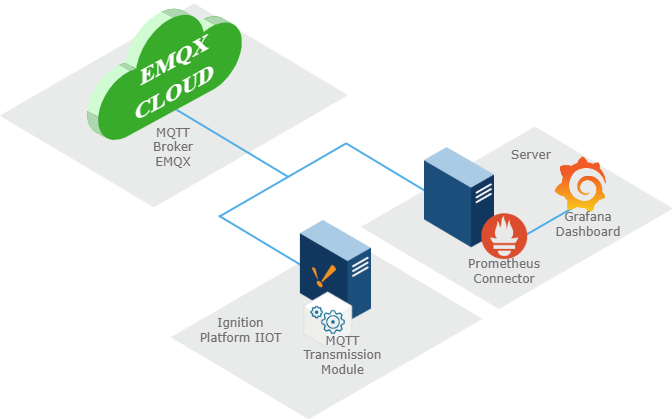
\includegraphics[width=13cm]{Figuras/DiagramaGrafana}}
\caption{Arquitectura de Evaluación de Desempeño}
\label{fig:grafanaconexion}
\end{figure}



La Fig. \ref{fig:grafanaconexion} representa el diagrama de conexiones que permite la evaluación del desempeño de las métricas cualitativas previamente definidas. El flujo de información inicia en la plataforma IIoT Ignition al publicar información generada en la plataforma de entrenamiento hacia un broker MQTT, específicamente el servidor EMQX desplegado en la nube. Posteriormente, un servidor se encarga de consumir estos datos desde el broker y monitorear las métricas mediante su interfaz. Estas métricas son recolectadas por Prometheus, un sistema de monitoreo que realiza consultas periódicas a través de la API del broker, almacenando los resultados en series temporales. 
Finalmente, el visualizador industrial Grafana, se conecta a la base de datos de Prometheus y permite construir paneles interactivos para el análisis histórico, la supervisión en tiempo real y la configuración de alertas basadas en el comportamiento de las métricas del sistema. Esta integración garantiza una visualización eficiente del rendimiento dentro de la plataforma IIoT según las métricas que se describen a continuación.


\subsubsection{Gestión de Tópicos y Sesiones MQTT}

Este conjunto de métricas evalúa la eficiencia del sistema en cuanto a la administración de los tópicos (temas) y las sesiones activas dentro del broker MQTT. Los tópicos representan los canales por los cuales se publica o se suscribe información, y las sesiones reflejan las conexiones activas de los clientes. Una gestión eficiente de estos elementos es fundamental para garantizar un sistema escalable, ordenado y con bajo riesgo de colisiones o redundancias en la comunicación. Además, un número optimizado de suscripciones indica una arquitectura mejor estructurada y alineada con el modelo de datos jerárquico del UNS.

\begin{itemize}
    \item\textbf{deployment\_emqx\_metrics\_topics\_count:} Mide la cantidad total de tópicos activos en el broker EMQX. Cada tópico representa un canal lógico por el que se publican o se reciben mensajes. Un sistema jerárquicamente estructurado tiende a organizar estos tópicos de forma más ordenada y controlada, minimizando redundancias.

    \item\textbf{deployment\_emqx\_sessions\_count:} Corresponde al número de sesiones activas en el broker, es decir, las conexiones cliente-servidor que están intercambiando datos. Esta métrica permite inferir el número de dispositivos o servicios que están interactuando directamente con el broker.
    \item\textbf{deployment\_emqx\_metrics\_subscriptions\_count:} Indica cuántas suscripciones activas existen. Una suscripción ocurre cuando un cliente se registra para recibir los mensajes publicados en un tópico específico. 

\end{itemize}

\begin{figure}[H]
\centerline{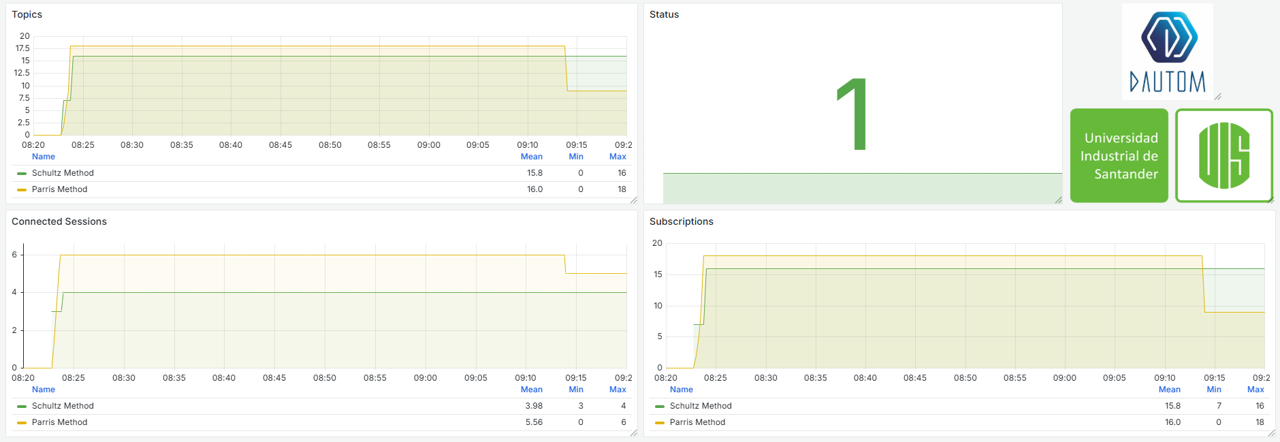
\includegraphics[width=20cm]{Figuras/gf_topics.png}}
\caption{Test de Gestión de Tópicos y Sesiones MQTT}
\label{fig:gf_topics}
\end{figure}

En Grafana se presentan los paneles de visualización con las series temporales como se muestra en la Fig. \ref{fig:gf_topics}. Allí se observan las métricas de gestión de tópicos y sesiones y se distinguen los resultados obtenidos mediante la técnica de Schultz (color verde) y los de la técnica de Parris (color amarillo). Además, se incluyen estadísticas relevantes derivadas del monitoreo continuo para contrastar el comportamiento de ambas arquitecturas.


\begin{table}[H]
\centering
\begin{tabular}{|c|c|c|}
\hline
\textbf{Métrica} & \textbf{Schultz} & \textbf{Parris} \\
\hline
\hspace{30pt}Tópicos\hspace{30pt} &
\hspace{30pt}16\hspace{30pt} & 
\hspace{30pt}18\hspace{30pt} \\
\hline
\hspace{30pt}Sesiones Conectadas\hspace{30pt} &
\hspace{30pt}4\hspace{30pt} & 
\hspace{30pt}6\hspace{30pt} \\
\hline
\hspace{30pt}Suscripciones\hspace{30pt} &
\hspace{30pt}16\hspace{30pt} & 
\hspace{30pt}18\hspace{30pt} \\
\hline
\end{tabular}
\caption{Comparación de Gestión de Tópicos y Sesiones MQTT}
\label{topics_com}
\end{table}



En la comparación de resultados entre las arquitecturas de Schultz y Parris, se observa un comportamiento consistente: Schultz presenta menores valores en las tres métricas como se evidencia en la Tabla \ref{topics_com}. Estos resultados evidencian una arquitectura más contenida y organizada por parte de Schultz. Al estructurar el UNS en distintos niveles jerárquicos, Schultz logra distribuir la responsabilidad de publicación y suscripción, reduciendo la concentración de carga en un único punto. En cambio, Parris, al centralizar toda la información en un solo broker, incrementa inevitablemente la cantidad de tópicos y sesiones necesarias para administrar la misma cantidad de datos, lo que puede dificultar la trazabilidad y escalabilidad del sistema.



\subsubsection{Gestión de Autenticaciones y Autorizaciones}


Este conjunto de métricas permite evaluar el comportamiento del sistema en relación con los procesos de autenticación y autorización de los clientes que interactúan con el broker MQTT. Estas operaciones son fundamentales para garantizar la seguridad, el control de acceso y la gestión eficiente de identidades dentro de arquitecturas IIoT. Analizar estas métricas proporciona una visión clara del volumen de autenticaciones realizadas, las solicitudes de autorización recibidas y las operaciones exitosas de control de acceso como se observa en la Fig.\ref{fig:gf_auten}, permitiendo detectar patrones o posibles vulnerabilidades. 

\begin{itemize}
    \item \textbf{deployment\_emqx\_metrics\_authentication\_success:} Representa el número total de autenticaciones exitosas realizadas por los clientes hacia el broker. Esta métrica es crítica para entender la cantidad de conexiones autenticadas correctamente durante el periodo de evaluación.
    
    \item \textbf{deployment\_emqx\_metrics\_client\_authorize:} Indica la cantidad de solicitudes de autorización recibidas por el broker por parte de los clientes autenticados. Cada vez que un cliente intenta publicar o suscribirse a un tópico, se genera una solicitud que debe ser autorizada, dependiendo de las políticas de control de acceso configuradas.
    
    \item \textbf{deployment\_emqx\_metrics\_authorization\_allow:} Refleja cuántas de esas solicitudes de autorización fueron permitidas según las reglas del sistema. Este valor debe correlacionarse estrechamente con la métrica anterior, y un alto valor sugiere que la mayoría de las operaciones solicitadas por los clientes fueron válidas y seguras.
\end{itemize}

\begin{figure}[h]
\centerline{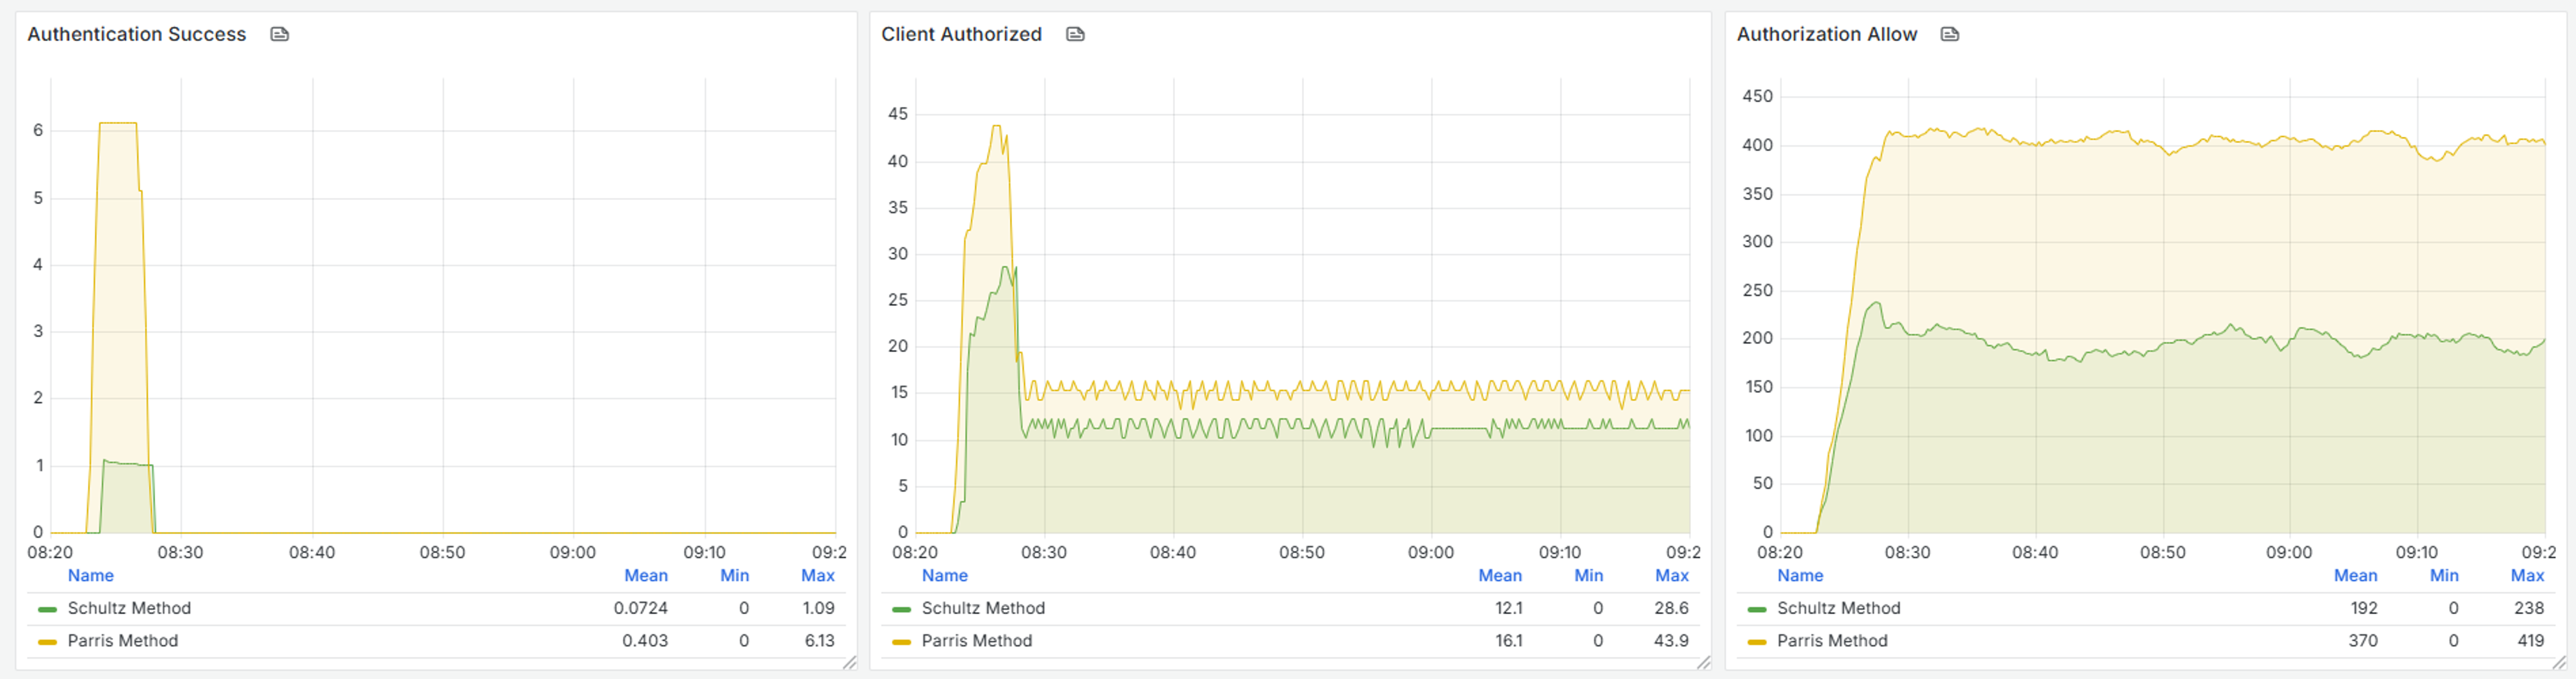
\includegraphics[width=20cm]{Figuras/gf_auten.png}}
\caption{Test de Gestión de Autenticaciones y Autorizaciones}
\label{fig:gf_auten}
\end{figure}


En la evaluación de las métricas relacionadas con autenticación y autorización, se evidencian diferencias notables entre las arquitecturas. La técnica de Parris presentó un mayor número de autenticaciones exitosas como se describe en la tabla \ref{auten_com}. Este comportamiento está directamente relacionado con su arquitectura centralizada, donde todos los clientes deben autenticarse y autorizarse directamente contra un único broker. Esta concentración genera un volumen más alto de operaciones en el punto central, aumentando la complejidad de gestión y potenciales cuellos de botella.

\begin{table}[H]
\centering
\begin{tabular}{|c|c|c|}
\hline
\textbf{Métrica} & \textbf{Schultz} & \textbf{Parris} \\
\hline
\hspace{30pt}Autenticaciones Exitosas\hspace{30pt} &
\hspace{30pt}1\hspace{30pt} & 
\hspace{30pt}6\hspace{30pt} \\
\hline
\hspace{30pt}Clientes Autorizados\hspace{30pt} &
\hspace{30pt}12\hspace{30pt} & 
\hspace{30pt}16\hspace{30pt} \\
\hline
\hspace{30pt}Autorizaciones Permitidas\hspace{30pt} &
\hspace{30pt}192\hspace{30pt} & 
\hspace{30pt}370\hspace{30pt} \\
\hline
\end{tabular}
\caption{Comparación de Gestión de Autenticaciones y Autorizaciones}
\label{auten_com}
\end{table}


Por su parte, la técnica de Schultz, al implementar una arquitectura jerárquica con múltiples niveles de brokers distribuidos, logra desacoplar el tráfico de autenticación, permitiendo que muchas de estas operaciones ocurran de forma intermedia antes de llegar al broker principal. Esto reduce la cantidad de accesos directos y mejora la segmentación de seguridad. Aunque sus métricas reflejan un menor volumen de eventos, este comportamiento implica una mayor eficiencia operativa y una arquitectura más segura y escalable, posicionando a Schultz como una mejor opción en entornos industriales que requieran control granular y tolerancia a fallos.


\subsubsection{Flujo de Datos}
Estas métricas están orientadas a evaluar el volumen de datos que circula a través del broker MQTT durante el funcionamiento de cada arquitectura, permitiendo cuantificar tanto la entrada como la salida de información del sistema a partir de tasas de transferencia promedio por segundo y por minuto. La Fig.\ref{fig:gf_bytes} permite observar con mayor claridad el comportamiento del flujo de datos en escalas de tiempo relevantes para operaciones industriales.

Estas métricas son fundamentales para entender el rendimiento de red y la eficiencia en el intercambio de datos entre productores (Ignition) y consumidores (cliente). Un flujo constante y bien distribuido es indicativo de una arquitectura optimizada tanto para el tráfico entrante como saliente, aspecto esencial en entornos IIoT donde grandes volúmenes de datos deben ser procesados en tiempo real sin generar obstrucciones.

\begin{figure}[H]
\centerline{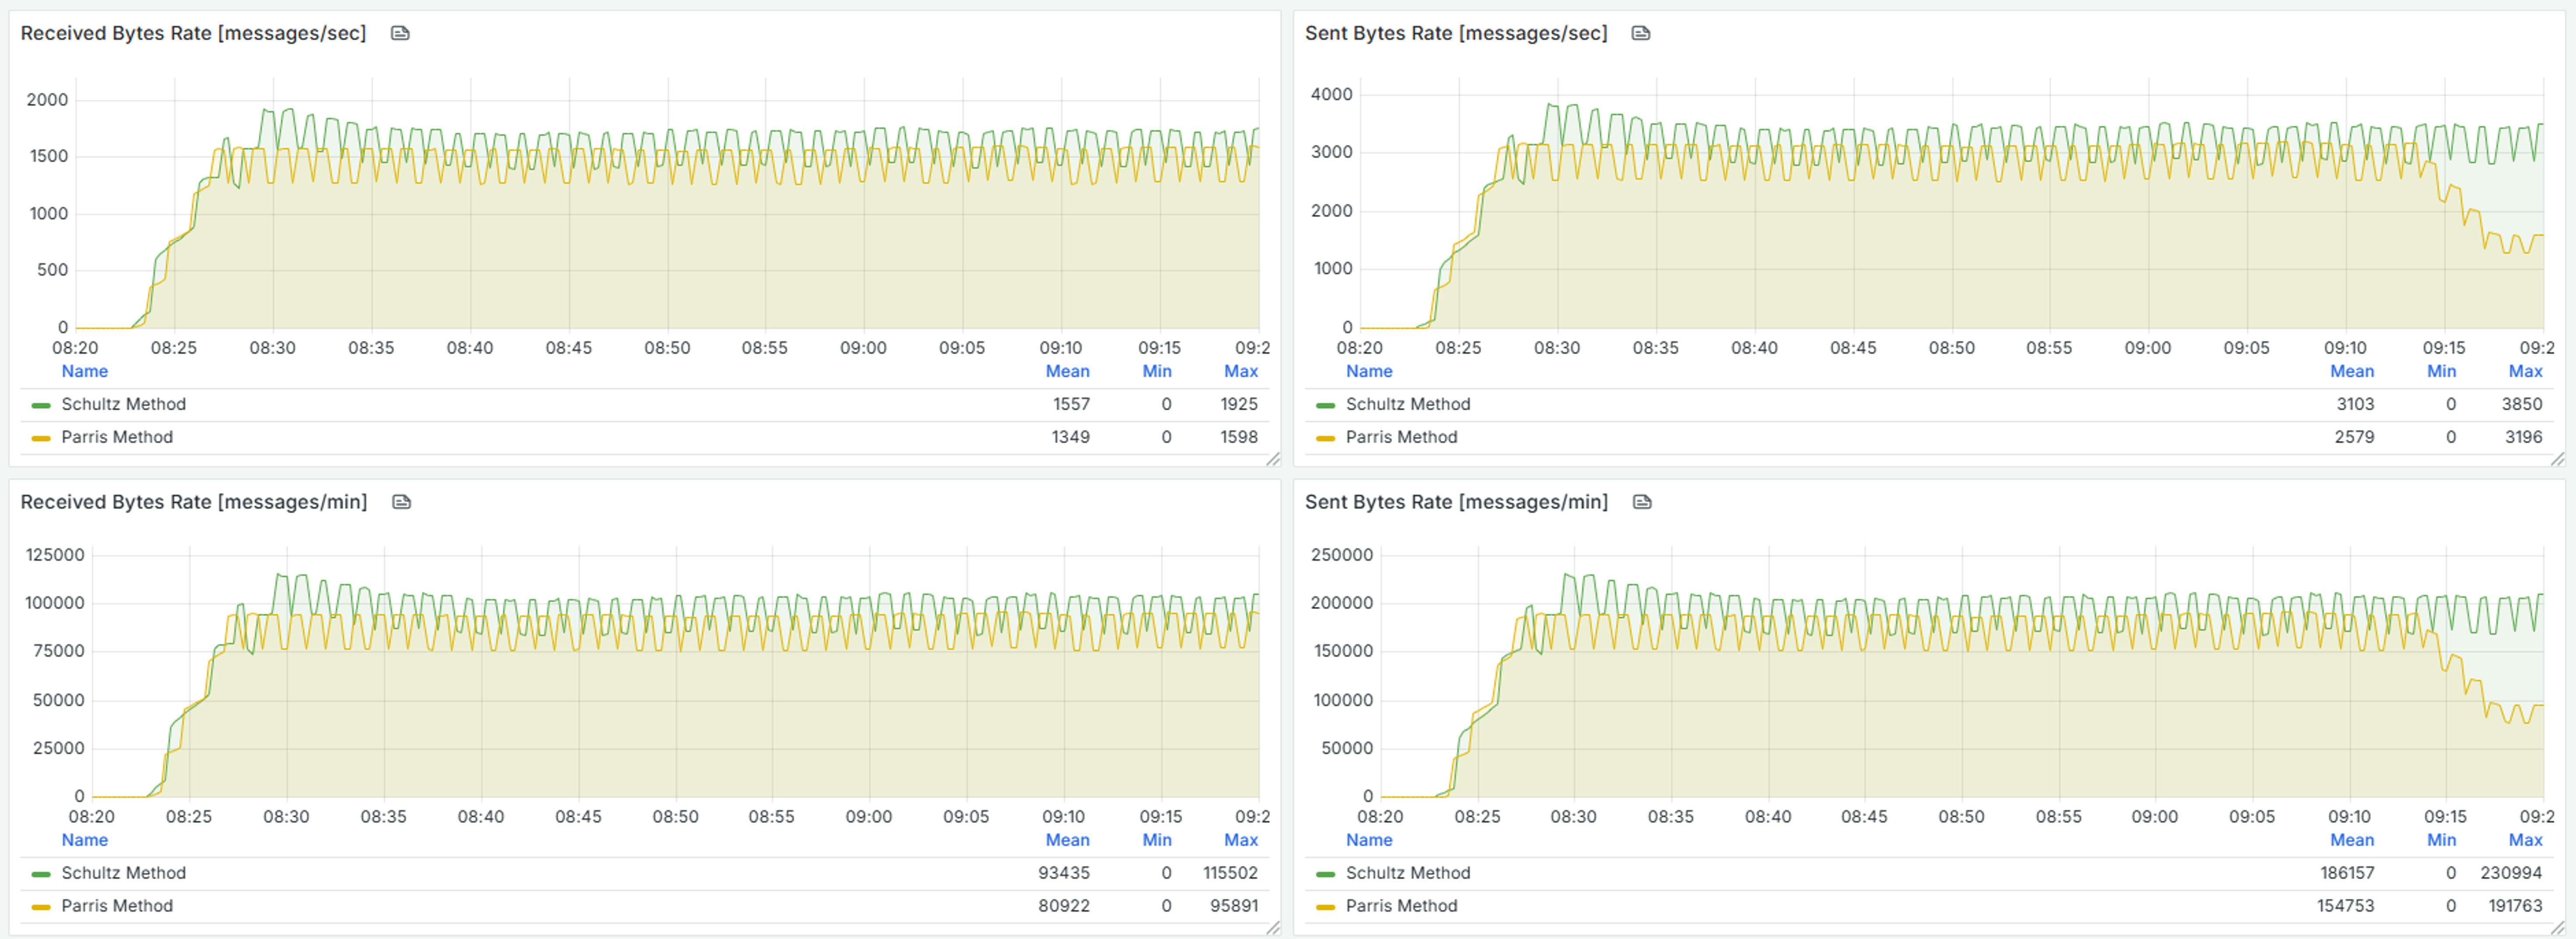
\includegraphics[width=20cm]{Figuras/gf_bytes.png}}
\caption{Test de Flujo de Datos}
\label{fig:gf_bytes}
\end{figure}


\begin{itemize}
    \item \textbf{deployment\_emqx\_metrics\_bytes\_received:} Mide la tasa de bytes recibidos por el broker, calcula la cantidad promedio de bytes recibidos por segundo en ese lapso, proporcionando una visión precisa de la cantidad de datos que el broker recibe desde las plataformas IIoT o dispositivos conectados.
    
    \item \textbf{deployment\_emqx\_metrics\_bytes\_sent:}  Similar a la métrica anterior, pero en este caso se mide la cantidad de bytes enviados por el broker a los clientes conectados para observar la salida de datos hacia las aplicaciones que consumen la información.
    
    \item \textbf{deployment\_emqx\_metrics\_bytes\_received*60:} Esta métrica es similar a la primera, pero escalada a bytes por minuto. Multiplicando la tasa por 60 se obtiene la cantidad total de bytes recibidos en un minuto para facilitar la interpretación de la cantidad de datos en un tiempo mayor y así planificar capacidades de la red.

    \item \textbf{deployment\_emqx\_metrics\_bytes\_sent*60:} Nuevamente, esta métrica mide la tasa de bytes enviados por el broker, pero escalada a bytes por minuto. Es útil para observar el volumen total de datos distribuidos hacia los clientes por minuto, brindando una visión más detallada del rendimiento en intervalos de tiempo más largos.
        
\end{itemize}


Los valores reportados para la tasa de datos recibidos indican que la técnica de Schultz alcanzó una media de 1.557 bytes/seg, frente a los 1.349 bytes/seg obtenidos por Parris como se compara en la tabla \ref{bytes_com} lo que demuestra que Schultz maneja una mayor cantidad de información tanto de entrada como de salida.

\begin{table}[H]
\centering
\begin{tabular}{|c|c|c|}
\hline
\textbf{Métrica} & \textbf{Schultz} & \textbf{Parris} \\
\hline
\hspace{30pt}Bytes Recibidos por Segundo\hspace{30pt} &
\hspace{30pt}1557\hspace{30pt} & 
\hspace{30pt}1349\hspace{30pt} \\
\hline
\hspace{30pt}Bytes Enviados por Segundo\hspace{30pt} &
\hspace{30pt}3103\hspace{30pt} & 
\hspace{30pt}2579\hspace{30pt} \\
\hline
\hspace{30pt}Bytes Recibidos por Minuto\hspace{30pt} &
\hspace{30pt}93435\hspace{30pt} & 
\hspace{30pt}80922\hspace{30pt} \\
\hline
\hspace{30pt}Bytes Enviados por Minuto\hspace{30pt} &
\hspace{30pt}186157\hspace{30pt} & 
\hspace{30pt}154753\hspace{30pt} \\
\hline
\end{tabular}
\caption{Comparación de Flujo de Datos}
\label{bytes_com}
\end{table}


Esta diferencia refleja cómo la arquitectura jerárquica y segmentada de Schultz permite un procesamiento y redistribución de datos más robusto, especialmente al escalar el sistema. Pese a su mayor complejidad en integración, Schultz optimiza el flujo de datos a través de sus múltiples niveles, evitando cuellos de botella. En cambio, aunque la técnica de Parris es más sencilla de integrar, su enfoque centralizado limita el rendimiento general cuando el volumen de datos aumenta. Esto convierte a Schultz en la opción más sólida para escenarios donde se espera alta densidad de tráfico o expansión futura del sistema.




\subsubsection{Gestión de Clientes}

Estas métricas se enfocan en la interacción de los clientes con el broker. Las métricas clave incluyen el número de conexiones establecidas por los clientes y la cantidad de autorizaciones que reciben para interactuar con el broker. Estos indicadores son fundamentales para medir la carga de trabajo del sistema, la eficiencia en la gestión de clientes y la efectividad de los mecanismos de autenticación y autorización. En términos generales, un análisis de estas métricas permite evaluar la capacidad de la infraestructura para manejar múltiples clientes y la velocidad con que se gestionan sus conexiones y autorizaciones. Los resultados se pueden evidenciar en la Fig.\ref{fig:gf_clients}.

\begin{itemize}
    \item \textbf{deployment\_emqx\_metrics\_client\_connect:} Esta métrica mide el número de conexiones de clientes al broker durante el intervalo de tiempo. Representa la cantidad de clientes que logran establecer una conexión exitosa con el broker.

    \item \textbf{deployment\_emqx\_metrics\_client\_authorize:} Mide el número de autorizaciones realizadas para los clientes durante un intervalo de tiempo determinado. Cada vez que un cliente es autenticado y autorizado para acceder a los servicios del broker, esta métrica incrementa.

\end{itemize}

\begin{figure}[H]
\centerline{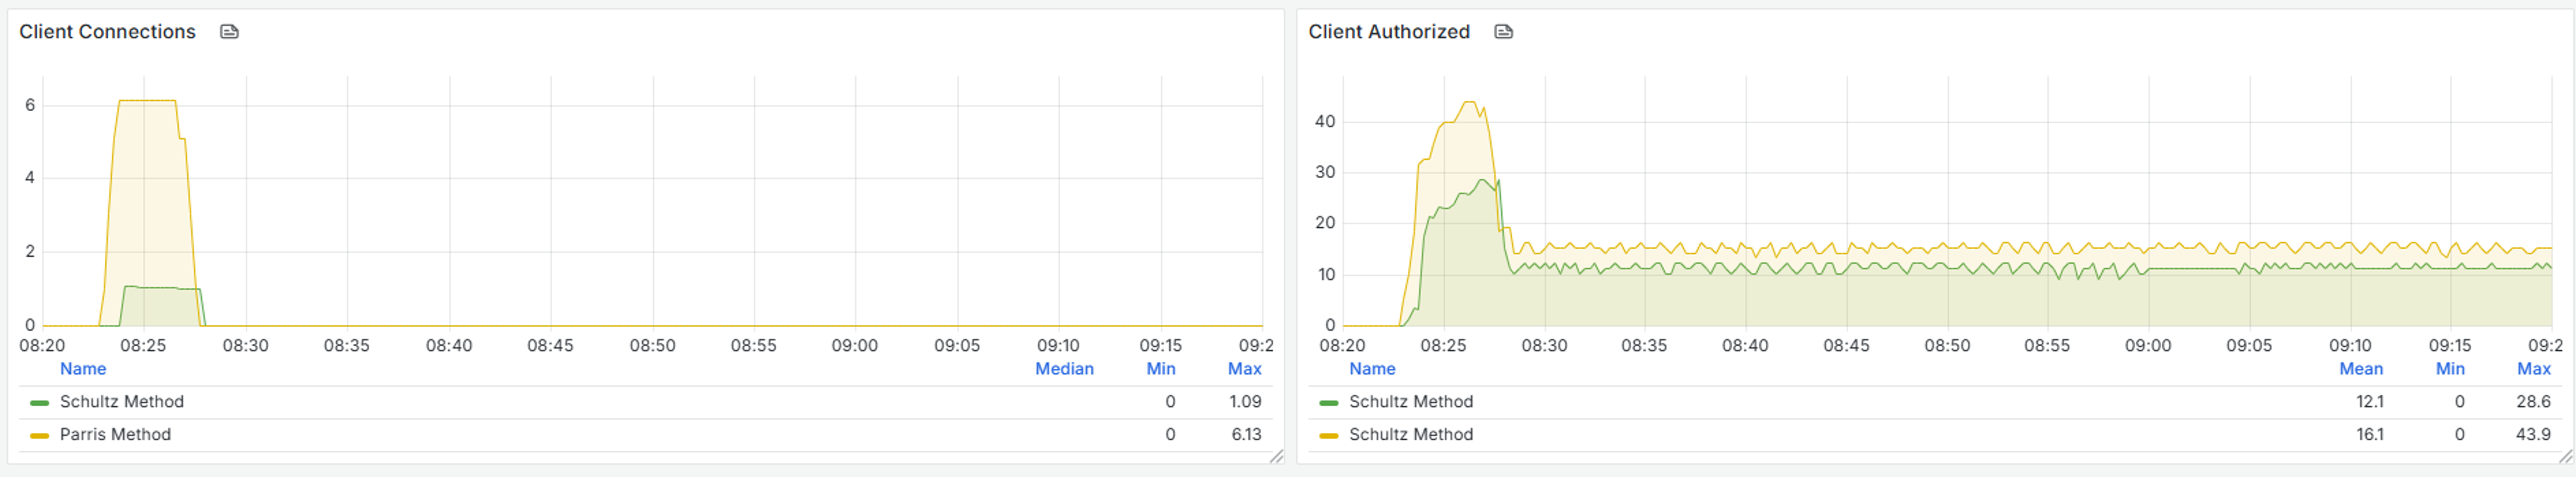
\includegraphics[width=20cm]{Figuras/gf_clients.png}}
\caption{Test de Gestión de Clientes}
\label{fig:gf_clients}
\end{figure}

Los resultados obtenidos en la tabla \ref{clients_com} revelan que la técnica de Schultz muestra una conexión significativamente menor con solo 1 cliente conectado durante el periodo de prueba en comparación con los 6 clientes de Parris. En términos de autorización, Schultz presenta 12 autorizaciones, mientras que Parris alcanza las 16, lo que sugiere que la técnica de Parris maneja una mayor cantidad de clientes conectados y autorizados dentro de los mismos intervalos de tiempo.

\begin{table}[H]
\centering
\begin{tabular}{|c|c|c|}
\hline
\textbf{Métrica} & \textbf{Schultz} & \textbf{Parris} \\
\hline
\hspace{30pt}Clientes Conectados\hspace{30pt} &
\hspace{30pt}1\hspace{30pt} & 
\hspace{30pt}6\hspace{30pt} \\
\hline
\hspace{30pt}Clientes Autorizados\hspace{30pt} &
\hspace{30pt}12\hspace{30pt} & 
\hspace{30pt}16\hspace{30pt} \\
\hline
\end{tabular}
\caption{Comparación de Gestión de Clientes}
\label{clients_com}
\end{table}


En términos generales, estos resultados indican que la técnica de Parris logra gestionar un mayor número de clientes simultáneamente en comparación con Schultz, lo que podría estar relacionado con su arquitectura centralizada que permite una gestión más sencilla de las conexiones y autorizaciones de clientes. Sin embargo, la técnica de Schultz podría ser más adecuada para escenarios donde la gestión de clientes se realiza de manera más autónoma en distintas áreas, lo cual podría generar una carga menor en el broker central.





\subsubsection{Gestión de Mensajes}

Este conjunto de métricas se centra en la actividad relacionada con el tráfico de mensajes dentro del broker. Evalúa tanto la recepción como el envío de mensajes, así como la frecuencia con la que los mensajes son publicados. Estas métricas son esenciales para entender el rendimiento de las arquitecturas IIoT en términos de comunicación, ya que permiten cuantificar la carga de datos que se transmite a través del sistema. Además, ayudan a identificar bloqueos en el flujo de información y permite evaluar la eficiencia del manejo del tráfico de mensajes bajo distintos esquemas de arquitectura.


\begin{itemize}
    \item \textbf{deployment\_emqx\_received\_msg\_rate:} Tasa promedio de mensajes recibidos para indicar cuántos mensajes el broker recibe en promedio en cada segundo dentro de esa ventana temporal.

    \item \textbf{deployment\_emqx\_sent\_msg\_rate:} Tasa promedio de mensajes enviados para reflejar la frecuencia con la que el broker distribuye mensajes a los clientes suscritos.

    \item \textbf{deployment\_emqx\_received\_msg\_rate* 60}: Proyección del total de mensajes recibidos por minuto. Se obtiene multiplicando la tasa por segundo por 60 para obtener una métrica más intuitiva a escala de minutos.

    \item \textbf{deployment\_emqx\_sent\_msg\_rate * 60:} Tasa de mensajes enviados por minuto, derivada del mismo procedimiento. Proporciona una mejor apreciación de la actividad total en el sistema durante períodos más largos.

    \item \textbf{deployment\_emqx\_metrics\_messages\_publish:} Mide la tasa de publicación de mensajes, es decir, la cantidad de mensajes nuevos que son publicados al broker en promedio por segundo durante el intervalo de tiempo.

\end{itemize}

\begin{figure}[H]
\centerline{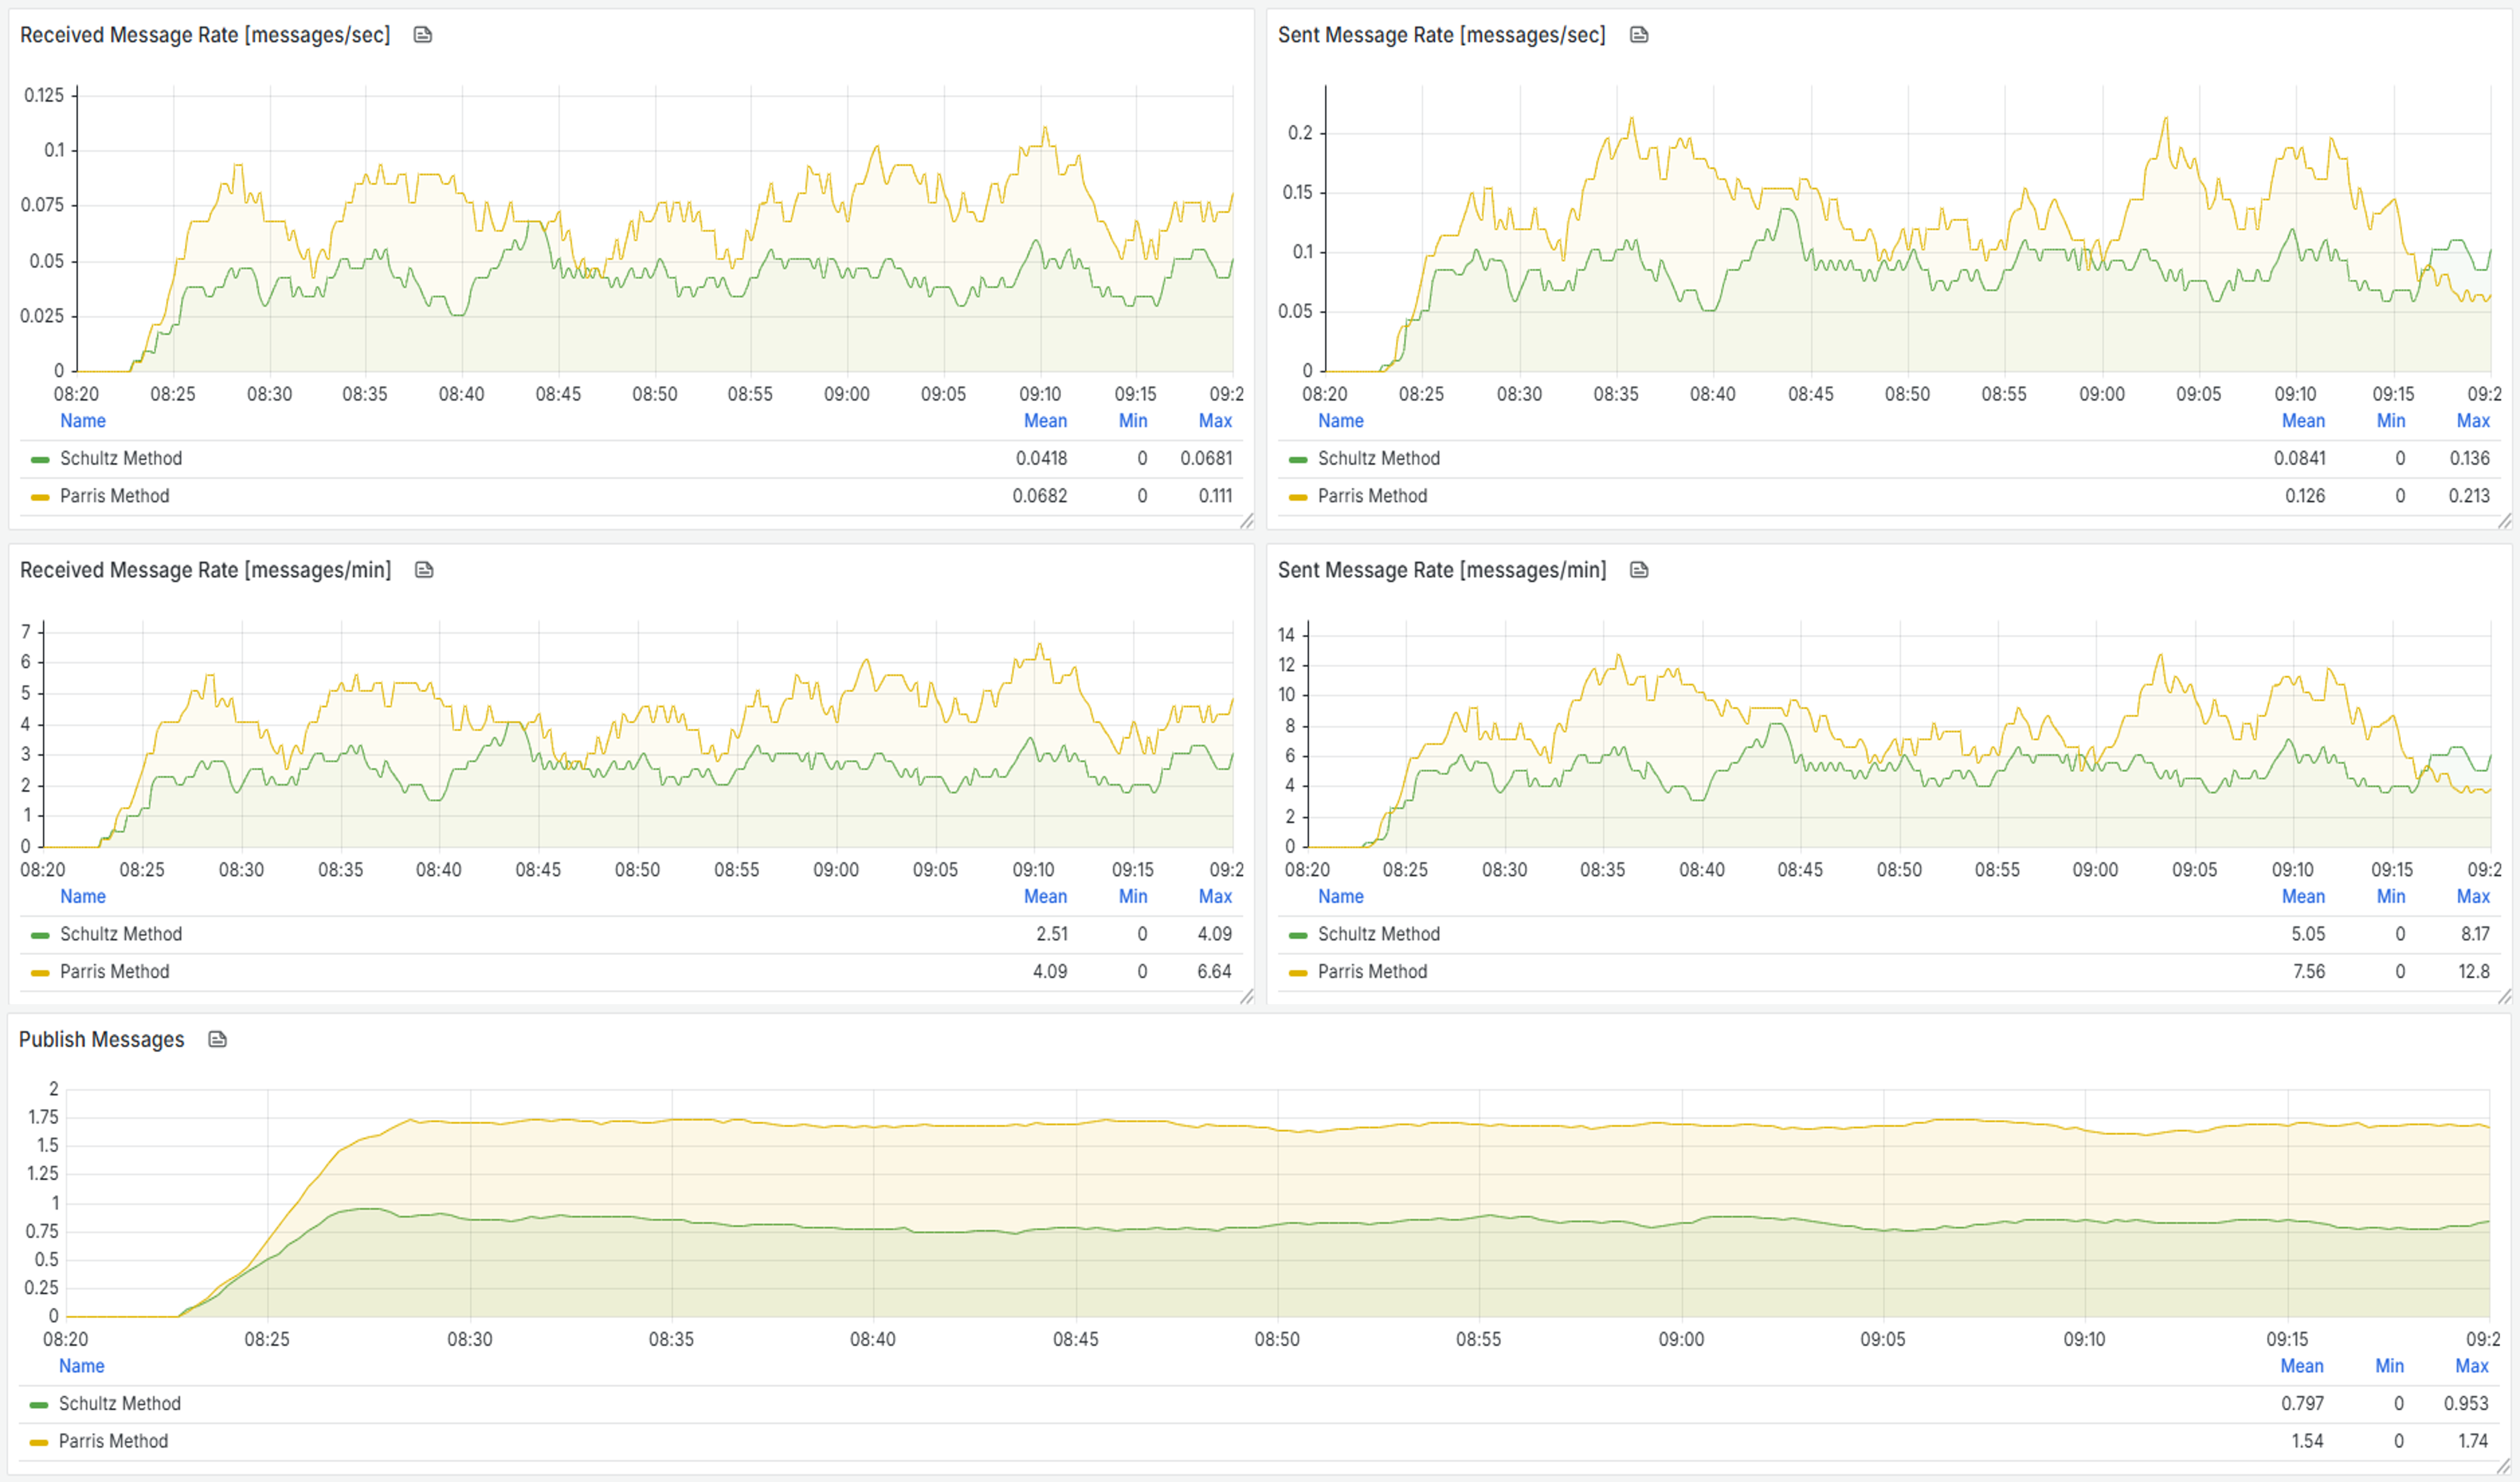
\includegraphics[width=20cm]{Figuras/gf_messages.png}}
\caption{Test de Gestión de Mensajes}
\label{fig:gf_messages}
\end{figure}


En la Fig. \ref{fig:gf_messages} se observan los resultado de la gestión de mensajes en cada una de las métricas definidas. Al comparar ambas arquitecturas, se observa que Parris mantiene una tasa superior tanto en recepción como en envío de mensajes. Los resultados de cada una de las tasas de mensajería se muestran en la tabla \ref{messages_com} a continuación.

\begin{table}[H]
\centering
\begin{tabular}{|c|c|c|}
\hline
\textbf{Métrica} & \textbf{Schultz} & \textbf{Parris} \\
\hline
\hspace{30pt}Mensajes Recibidos por Segundo\hspace{30pt} &
\hspace{30pt}0.0588\hspace{30pt} & 
\hspace{30pt}0.0763\hspace{30pt} \\
\hline
\hspace{30pt}Mensajes Enviados por Segundo\hspace{30pt} &
\hspace{30pt}0.124\hspace{30pt} & 
\hspace{30pt}0.167\hspace{30pt} \\
\hline
\hspace{30pt}Mensajes Recibidos por Minuto\hspace{30pt} &
\hspace{30pt}3.53\hspace{30pt} & 
\hspace{30pt}4.58\hspace{30pt} \\
\hline
\hspace{30pt}Mensajes Enviados por Minuto\hspace{30pt} &
\hspace{30pt}7.45\hspace{30pt} & 
\hspace{30pt}10\hspace{30pt} \\
\hline
\hspace{30pt}Mensajes Publicados\hspace{30pt} &
\hspace{30pt}0.797\hspace{30pt} & 
\hspace{30pt}1.54\hspace{30pt} \\
\hline
\end{tabular}
\caption{Comparación de Gestión de Mensajes}
\label{messages_com}
\end{table}


Estos resultados sugieren que Parris facilita una mayor actividad de mensajería dentro del mismo intervalo de tiempo. Esta diferencia se atribuye al enfoque centralizado de la arquitectura, que permite una difusión más rápida y directa de los mensajes, sin requerir pasos intermedios de agregación o procesamiento. En contraste, la arquitectura Schultz, al segmentar jerárquicamente los niveles de información, puede introducir latencias naturales que impactan la tasa de publicación y distribución de mensajes, aunque podría estar optimizada para casos donde se priorice robustez o filtrado local. 

\subsubsection{Actividad de Paquetes}

Este último grupo comprende métricas orientadas a monitorear el volumen y comportamiento del tráfico de paquetes que circulan entre los clientes y el broker. A diferencia de las métricas de mensajes, que se enfocan en el contenido informativo que se transmite, las métricas de paquetes se centran en los distintos tipos de señales del protocolo MQTT que permiten establecer, mantener y finalizar las conexiones, así como realizar operaciones como suscripciones y publicaciones. 

Estas métricas son fundamentales para caracterizar el nivel de interacción entre clientes y el servidor, evaluar el rendimiento del canal de comunicación y detectar posibles cuellos de botella en la negociación del protocolo.\\~\\

\begin{itemize}
    \item \textbf{rate(deployment\_emqx\_metrics\_packets\_received):} Tasa de recepción de paquetes por segundo. Refleja el flujo constante de datos entrantes hacia el broker, incluyendo todos los tipos de paquetes MQTT.

    \item \textbf{rate(deployment\_emqx\_metrics\_packets\_sent):} Tasa de paquetes enviados por segundo. Mide la capacidad del broker para responder a los clientes o reenviar datos, útil para analizar la carga saliente.

    \item \textbf{increase(deployment\_emqx\_metrics\_packets\_received):} Incremento total de paquetes recibidos durante el intervalo de análisis. Indica la acumulación neta de tráfico entrante.

    \item \textbf{increase(deployment\_emqx\_metrics\_packets\_sent):} Incremento total de paquetes enviados en el periodo observado. Complementa la métrica anterior para reflejar la magnitud de la actividad bidireccional.

    \item \textbf{deployment\_emqx\_metrics\_packets\_subscribe\_received:} Cantidad de paquetes SUBSCRIBE recibidos. Representa solicitudes de suscripción a tópicos por parte de los clientes.

    \item \textbf{deployment\_emqx\_metrics\_packets\_connect:} Número de paquetes CONNECT. Corresponde a los intentos de los clientes por establecer una conexión con el broker.

    \item \textbf{deployment\_emqx\_metrics\_packets\_pingreq\_received:} Cantidad de paquetes PINGREQ recibidos. Usados por los clientes para mantener viva la conexión, especialmente en períodos de inactividad de datos.

\end{itemize}

\begin{figure}[H]
\centerline{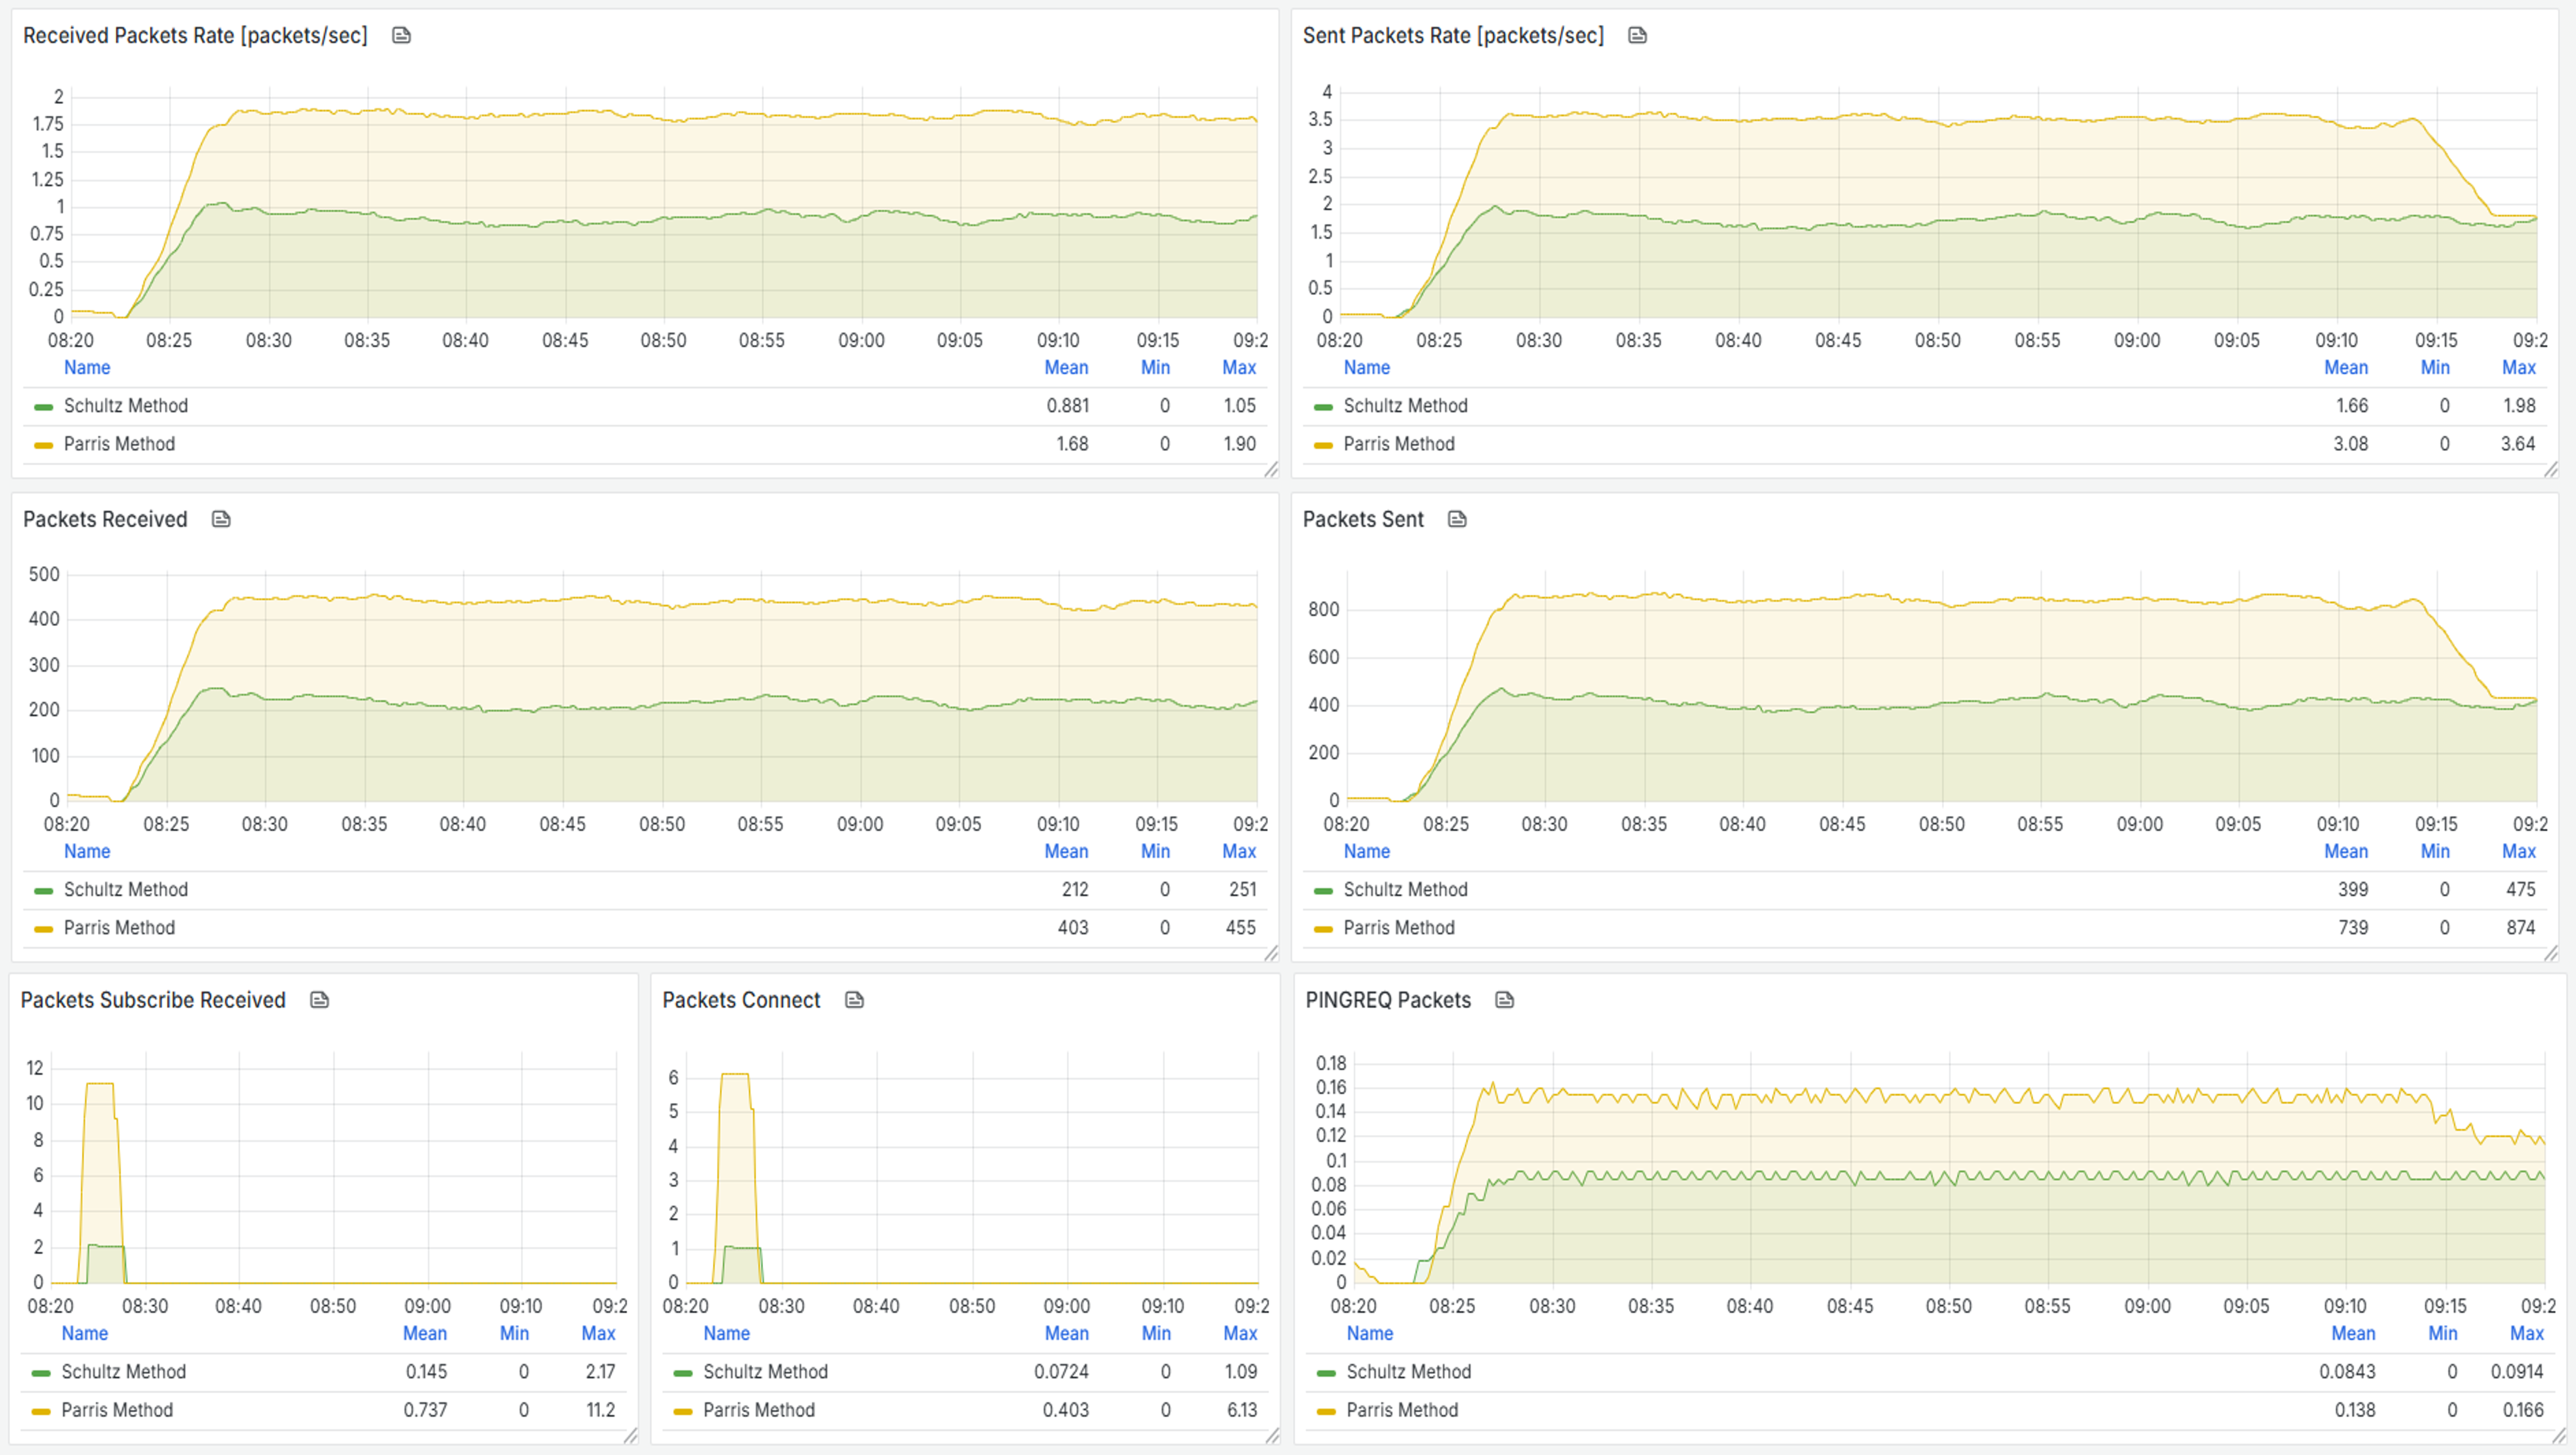
\includegraphics[width=20cm]{Figuras/gf_packets.png}}
\caption{Test de Actividad de Paquetes}
\label{fig:gf_packets}
\end{figure}

Los resultados presentados en la Tabla \ref{packets_com} muestran que la técnica Parris genera una actividad significativamente más intensiva en el intercambio de paquetes MQTT, con una mayor tasa de transmisión y recepción, así como un número más elevado de mensajes asociados a conexiones, suscripciones y mantenimiento de sesión. Este comportamiento indica una mayor frecuencia de interacción entre clientes y servidor, lo que puede traducirse en una respuesta más rápida ante eventos y cambios en el sistema. Tal dinámica resulta especialmente útil en entornos que requieren actualizaciones de estado en tiempo real o una sincronización continua entre múltiples dispositivos.

\begin{table}[H]
\centering
\begin{tabular}{|c|c|c|}
\hline
\textbf{Métrica} & \textbf{Schultz} & \textbf{Parris} \\
\hline
\hspace{30pt}Paquetes Recibos por Segundo\hspace{30pt} &
\hspace{30pt}0.881\hspace{30pt} & 
\hspace{30pt}1.68\hspace{30pt} \\
\hline
\hspace{30pt}Paquetes Enviados por Segundo\hspace{30pt} &
\hspace{30pt}1.66\hspace{30pt} & 
\hspace{30pt}3.08\hspace{30pt} \\
\hline
\hspace{30pt}Paquetes Payload Recibidos\hspace{30pt} &
\hspace{30pt}212\hspace{30pt} & 
\hspace{30pt}403\hspace{30pt} \\
\hline
\hspace{30pt}Paquetes Payload Enviados\hspace{30pt} &
\hspace{30pt}399\hspace{30pt} & 
\hspace{30pt}739\hspace{30pt} \\
\hline
\hspace{30pt}Paquetes de Subscripción Recibidos\hspace{30pt} &
\hspace{30pt}2\hspace{30pt} & 
\hspace{30pt}11\hspace{30pt} \\
\hline
\hspace{30pt}Paquetes de Conexión\hspace{30pt} &
\hspace{30pt}1\hspace{30pt} & 
\hspace{30pt}6\hspace{30pt} \\
\hline
\hspace{30pt}Paquetes PINGREQ\hspace{30pt} &
\hspace{30pt}0.0843\hspace{30pt} & 
\hspace{30pt}0.138\hspace{30pt} \\
\hline
\end{tabular}
\caption{Comparación de Actividad de Paquetes}
\label{packets_com}
\end{table}


En contraste, la técnica de Schultz genera un tráfico de paquetes más moderado con una comunicación con menor intensidad. Esta característica representa una ventaja en términos de eficiencia en el uso de la red y consumo de recursos, especialmente en entornos con conectividad limitada o donde se prioriza la estabilidad sobre la inmediatez.No obstante, considerando la mayor capacidad de respuesta y el flujo de información sostenido que ofrece la técnica Parris según estas métricas, sería recomendable su implementación en contextos donde la criticidad operativa y la necesidad de monitoreo continuo sean factores clave.



\subsection {Síntesis y Recomendaciones de Implementación}

El análisis comparativo entre las técnicas Schultz y Parris, sustentado en las métricas cualitativas y cuantitativas, permite establecer un panorama integral sobre su desempeño y aplicabilidad en distintos entornos industriales y académicos. La tabla \ref{all_com} refleja que la técnica Schultz mostró un rendimiento más favorable en aspectos como la resiliencia, seguridad, facilidad de implementación, escalabilidad y eficiencia en la gestión de autenticaciones, clientes, tópicos y sesiones MQTT. Esto sugiere que Schultz es adecuada para entornos donde se prioriza la estabilidad operativa, la predictibilidad del comportamiento del sistema, y donde las capacidades de despliegue deben ser rápidas y confiables. En contraste, la técnica Parris demostró fortalezas en dimensiones como integración con otros servicios, flexibilidad para adaptarse a distintos escenarios de comunicación, y un desempeño más eficiente en la gestión dinámica de mensajes y paquetes. Estos resultados la posicionan como una alternativa más apropiada para arquitecturas en evolución, entornos distribuidos con alta interacción entre componentes, o soluciones que requieren una rápida adaptabilidad a cambios en el sistema.

\begin{table}[H]
\centering
\begin{tabular}{|c|c|c|}
\hline
\textbf{Métrica} & \textbf{Schultz} & \textbf{Parris} \\
\hline

\hspace{20pt}Integracion\hspace{20pt} &
\hspace{20pt}{\color{red}\ding{55}}\hspace{20pt} & 
\hspace{2pt}{\color{green}\ding{51}}\hspace{20pt}\\
\hline

\hspace{20pt}Resiliencia\hspace{20pt} &
\hspace{20pt}{\color{green}\ding{51}}\hspace{20pt} & 
\hspace{20pt}{\color{red}\ding{55}}\hspace{20pt} \\
\hline

\hspace{20pt}Flexibilidad\hspace{20pt} &
\hspace{20pt}{\color{red}\ding{55}}\hspace{20pt} & 
\hspace{2pt}{\color{green}\ding{51}}\hspace{20pt}\\
\hline

\hspace{20pt}Seguridad\hspace{20pt} &
\hspace{20pt}{\color{green}\ding{51}}\hspace{20pt} & 
\hspace{20pt}{\color{red}\ding{55}}\hspace{20pt} \\
\hline

\hspace{20pt}Implementación\hspace{20pt} &
\hspace{20pt}{\color{green}\ding{51}}\hspace{20pt} & 
\hspace{20pt}{\color{red}\ding{55}}\hspace{20pt} \\
\hline

\hspace{20pt}Escalabilidad\hspace{20pt} &
\hspace{20pt}{\color{green}\ding{51}}\hspace{20pt} & 
\hspace{20pt}{\color{red}\ding{55}}\hspace{20pt} \\
\hline

\hspace{20pt}Gestion de Topicos y Sesiones MQTT \hspace{20pt} &
\hspace{20pt}{\color{green}\ding{51}}\hspace{20pt} & 
\hspace{20pt}{\color{red}\ding{55}}\hspace{20pt} \\
\hline

\hspace{20pt}Gestion de Autenticaciones y Autorizaciones\hspace{20pt} &
\hspace{20pt}{\color{green}\ding{51}}\hspace{20pt} & 
\hspace{20pt}{\color{red}\ding{55}}\hspace{20pt} \\
\hline

\hspace{20pt}Flujo de Datos\hspace{20pt} &
\hspace{20pt}{\color{green}\ding{51}}\hspace{20pt} & 
\hspace{20pt}{\color{red}\ding{55}}\hspace{20pt} \\
\hline

\hspace{20pt}Gestion de Clientes\hspace{20pt} &
\hspace{20pt}{\color{green}\ding{51}}\hspace{20pt} & 
\hspace{20pt}{\color{red}\ding{55}}\hspace{20pt} \\
\hline

\hspace{20pt}Gestion de Mensajes\hspace{20pt} &
\hspace{20pt}{\color{red}\ding{55}}\hspace{20pt} &
\hspace{20pt}{\color{green}\ding{51}}\hspace{20pt} \\
\hline

\hspace{20pt}Actividad de Paquetes\hspace{20pt} &
\hspace{20pt}{\color{red}\ding{55}}\hspace{20pt} &
\hspace{20pt}{\color{green}\ding{51}}\hspace{20pt} \\
\hline

\end{tabular}
\caption{Síntesis de Comparación entre Schultz y Parris}
\label{all_com}
\end{table}


En síntesis, Schultz se presenta como la opción más robusta y sencilla para implementaciones en ambientes críticos, controlados o con restricciones de seguridad y recursos, mientras que Parris resulta ideal para proyectos que buscan flexibilidad, interacción con múltiples sistemas y optimización en el flujo de datos, particularmente en fases de expansión tecnológica o integración con plataformas externas. La elección entre ambas dependerá entonces de la etapa del proyecto, la infraestructura disponible y los objetivos operativos del sistema.


